\section{Metodologia}

\subsection{Sistema massa–mola}

Utiliza-se um conjunto composto por suporte metálico, molas de diferentes constantes elásticas e massas calibradas. Cada massa é acoplada à extremidade inferior da mola, a qual é fixada ao suporte. A massa é então deslocada verticalmente e solta, iniciando oscilações. O tempo para 10 oscilações completas é registrado com cronômetro digital. O experimento é repetido com diferentes massas e molas.

A frequência de oscilação \(f\) é obtida por:

\begin{align*}
    f = \frac{1}{2\pi} \sqrt{\frac{k}{m}}
\end{align*}

A \cref{fig:massamola} apresenta o sistema massa–mola montado com massa pendurada.

\begin{figure}[H]
    \centering
    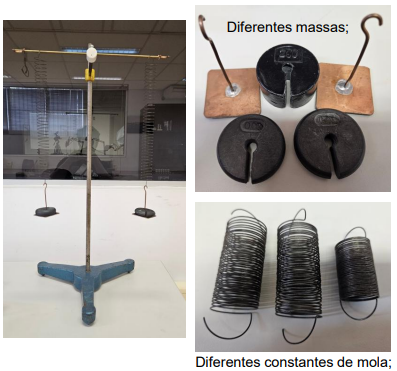
\includegraphics[width=0.35\linewidth]{fig/massamola.jpeg}
    \caption{Sistema massa–mola com massa acoplada à extremidade inferior da mola}
    \label{fig:massamola}
\end{figure}

\subsection{Pêndulo de Wilberforce}

O pêndulo de Wilberforce é constituído por uma mola helicoidal vertical e um cilindro metálico capaz de oscilar simultaneamente nos modos vertical e rotacional. A mola é fixada ao suporte superior, com o cilindro acoplado à sua extremidade. O sistema é iniciado com oscilação exclusivamente vertical, observando-se posteriormente o acoplamento com o movimento rotacional.

A \cref{fig:wilberforce} mostra o sistema no momento da oscilação.

\begin{figure}[H]
    \centering
    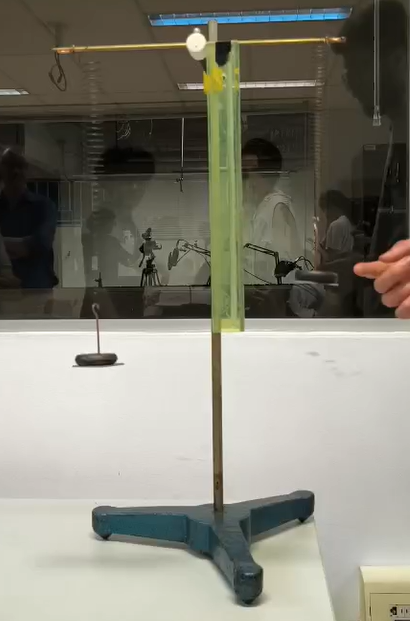
\includegraphics[width=0.35\linewidth]{fig/wilberforce.jpeg}
    \caption{Pêndulo de Wilberforce com cilindro oscilando vertical e angularmente}
    \label{fig:wilberforce}
\end{figure}

\subsection{Pêndulo de torção}

Utiliza-se um fio metálico fino, fixado na extremidade superior, com um cilindro metálico suspenso em sua extremidade inferior. O sistema realiza oscilações angulares em torno do eixo do fio. O tempo para 10 oscilações é registrado com cronômetro digital. O experimento é realizado em dois meios: ar e óleo. No segundo caso, o cilindro é parcialmente imerso.

A \cref{fig:torsao} mostra o pêndulo de torção parcialmente submerso no meio viscoso.

\begin{figure}[H]
    \centering
    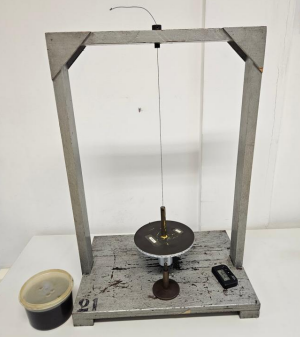
\includegraphics[width=0.35\linewidth]{fig/torsao.jpeg}
    \caption{Pêndulo de torção com cilindro parcialmente imerso em óleo}
    \label{fig:torsao}
\end{figure}

\subsection{Propagação de ondas em molas}

São utilizadas duas molas com diferentes rigidezes, dispostas horizontalmente sobre superfície plana. Ondas transversais e longitudinais são geradas por impulsos aplicados manualmente em uma extremidade da mola. Observam-se a propagação da perturbação, a formação de nós e os padrões de interferência.

A \cref{fig:ondas} apresenta uma mola com onda transversal em propagação.

\begin{figure}[H]
    \centering
    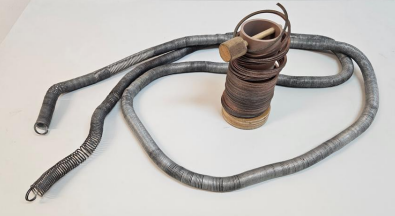
\includegraphics[width=0.35\linewidth]{fig/ondas.jpeg}
    \caption{Propagação de onda transversal em mola estendida horizontalmente}
    \label{fig:ondas}
\end{figure}

\subsection{Esfera vibrando}

Uma esfera metálica é acoplada a um excitador eletromecânico de frequência variável. A frequência é ajustada progressivamente até que padrões de ressonância sejam observados na superfície da esfera. São identificadas regiões nodais e antinodais.

A \cref{fig:esfera} ilustra a esfera no momento em que apresenta vibração ressonante.

\begin{figure}[H]
    \centering
    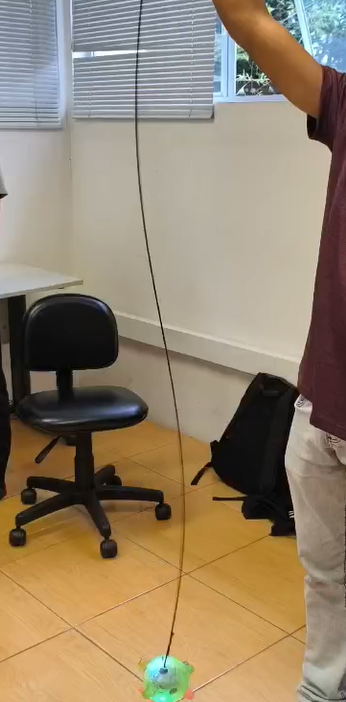
\includegraphics[width=0.35\linewidth]{fig/esfera.jpeg}
    \caption{Esfera acoplada a excitador vibrando em frequência ressonante}
    \label{fig:esfera}
\end{figure}
